\documentclass{beamer}


\usetheme{Warsaw}
\usecolortheme{crane}


\title{Partial Differentiation}                    %TODO: Add a title.
\subtitle{Mathematical Methods in the Physical Sciences}
\author{Steve Mazza}
\institute[Naval Postgraduate School]
{ 
    Naval Postgraduate School \\
    Monterey, CA \\
    
\includegraphics[height=3cm]{images/NPS_logo.jpg}
}
\date {SE3030, Winter/2014 \\ Quantitative Methods of Systems Engineering}
\subject{Quantitative Methods of Systems Engineering}


\begin{document}

\frame{\titlepage}


\frame {{Lorenz Attractor}
	\begin{center}
		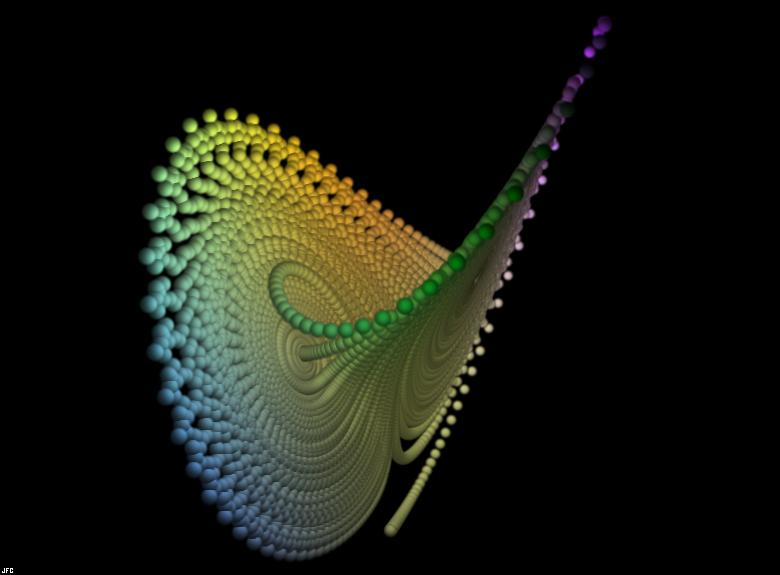
\includegraphics[width=0.8\textwidth]{images/LorenzBeads.jpg}
	\end{center}
}


\frame{{Introduction}
	\begin{block}{Definition}
		Derivatives of a multi-variable function where all variables are held fixed during differentiation except the variable of interest.
	\end{block}
	To denote this we write $\dfrac{\partial}{\partial y}$, generically.
	%TODO: Replace the following example with 4.1.12
	\begin{exampleblock}{Let $f(x,y) = x^{2}y^{3}$ , calculate $\dfrac{\partial f}{\partial x}(x,y)$}
		\begin{align*}
			g(x) &= x^{2}u^{3}, y=u \\
			\dfrac{dg}{dx}(x) &= 2b^{3}x \\
			\dfrac{\partial f}{\partial x}(x,y) &= 2xy^{3}, u=y
		\end{align*}
	\end{exampleblock}
}


\frame{{Power Series in Two Variables}
	Our standard power series expansions can be re-written as partial differential equations.
	\begin{block}{Definition}
		\[
			f(x,y) = \sum_{n=0}^{\infty}\dfrac{1}{n!}\left(h\dfrac{\partial}{\partial x}+k\dfrac{\partial}{\partial y}\right)^{n}f(a,b)
		\]
	\end{block}
	%TODO: work an example.
}


\frame{{Total Differentials}
	\begin{block}{Total Differentiation in 2 Variables}
		\[
			dz = \dfrac{\partial}{\partial x}dx+\dfrac{\partial}{\partial y}dy
		\]
	\end{block}
}


\frame{{Approximations Using Differentials}

}


\frame{{Chain Rule}
%	\begin{block}{Definition}
%		\[
%			dz = \dfrac{\partial z}{\partial x}dx+\dfrac{\partial z}{\partial y}dy
%		\]
%	\end{block}
	\begin{block}{In General}
		\[
			\dfrac{dy}{dx} = \dfrac{dy}{du}\dfrac{du}{dv}\dfrac{dv}{dx}
		\]
	\end{block}
	\begin{exampleblock}{Find $dy/dx$ if $y=$ ln sin$2x$}
		\begin{align*}
			\dfrac{dy}{dx} &= \dfrac{1}{\text{sin}2x}\cdot\dfrac{d}{dx}(\text{sin}2x) \\
			&= \dfrac{1}{\text{sin}2x}\cdot\text{cos}2x\cdot\dfrac{d}{dx}(2x) \\
			&= 2\text{cot}2x
		\end{align*}
	\end{exampleblock}
}


\frame{{Implicit Differentiation}

}


\frame{{Chain Rule (Redux)}
	We can extend our earlier examples of the Chain Rule where $z=f(x,y)$ where $x$ and $y$ were functions of $t$ by considering the case where $x$ and $y$ are two variables, $s$ and $t$.
		%TODO: Consider working 4.7.3
}


\frame{{Applications}

}


\begin{frame}{Questions?}
	\begin{center}
		
\includegraphics[width=.7\textwidth]{images/fin.png}
	\end{center}
\end{frame}

\end{document}
